\chapter{Background and Motivation}
\label{chap:background}

In this chapter I lay out the physics context of my work. We will define the framework we are testing, the standard model. We will expand on the details of the specific sector we are interested in - the flavour sector and the CKM matrix.

\section{Testing the Standard Model}

{\red{need to add: intro to discrete Lorentz symmetries

    mention how $SU(3)_C\times SU(2)_L \times U(1)_Y$ relates to electromagnetism via EWSB.

    include any stuff in Lenz's flavour physics lectures intro to SM that has been missed out here.

    maybe put QCD section in here, before the FCCC section (since I claim that QCD matrix elements cannot be computed with perturbation theory...)

    READING LIST:
    Lenz, Flavour physics lectures. 1812.11211, 1703.08170

    'The B-physics program' :https://www.ncbi.nlm.nih.gov/pmc/articles/PMC4737432/\#andp201500230-sec-0020title

    }}

The Standard Model of Particle Physics (SM) is, so far, the most successful theory for describing fundemental particles and their interactions. It is an effective Yang-Mills quantum field theory. It is most succinctly defined by listing it's symmetries, field content, and the irreducable representations (irreps) of the symmetries that those fields transform under.

The symmetries are the following. The Lorentz group $SO(3,1)$, the group of coordinate transformations that leave the Minkowski metric invariant, which can be decomposed into $SU(2)_l\times SU(2)_r$ ({\it{left-handed}} and {\it{right-handed}}). We denote an irrep as $(a,b)$ where $a$ is the $\sigma^z$ eigenvalue under $SU(2)_l$ transforms, and $b$ is that of $SU(2)_r$. Then there are internal local gauge symmetries:
\begin{align}
  SU(3)_C\times SU(2)_L \times U(1)_Y,
\end{align}
irreps of which we denote with $(x,y,z)$, where $x,y$ are the $SU(3)_C$ and $SU(2)_W$ irreps and $z$ is the charge under $U(1)_Y$.

The field content is: gauge bosons for each generator of the above gauge symmetries, each transforming in the adjoint of their corresponding symmetry and in the $(1/2,1/2)$ irrep of the Lorentz group, denoted $B_{\mu}$, $W_{\mu}$, $G_{\mu}$ respectively. There are 6 $SU(2)_L$ doublets in the $(1/2,0)$ Lorentz irrep;
\begin{align}
  Q_{1,2,3} =&
  \begin{pmatrix} u_L \\ d_L \end{pmatrix},
  \begin{pmatrix} c_L \\ s_L \end{pmatrix},
  \begin{pmatrix} t_L \\ b_L \end{pmatrix}
  \quad,\quad
  (\mathbf{3},\mathbf{2},1/6) \\
  L_{1,2,3} =&
  \begin{pmatrix} \nu_{e,L} \\ e_L \end{pmatrix},
  \begin{pmatrix} \nu_{\mu,L} \\ \mu_L \end{pmatrix},
  \begin{pmatrix} \nu_{\tau,L} \\ \tau_L \end{pmatrix}
  \quad,\quad
  (\mathbf{1},\mathbf{2},-1)
\end{align}
and 9 $SU(2)_W$ singlets in the $(0,1/2)$ Lorentz irrep;
\begin{align}
  u^R_{1,2,3} &= u_R, c_R, t_R\quad,\quad (\bar{\mathbf{3}},\mathbf{1},2/3) \\
  d^R_{1,2,3} &= d_R, s_R, b_R\quad,\quad (\bar{\mathbf{3}},\mathbf{1},-1/3) \\
  e^R_{1,2,3} &= e_R, \mu_R, \tau_R\quad,\quad (\mathbf{1},\mathbf{1},-1)
\end{align}
We have also listed the SM gauge irreps next to each definition. There is also in principle a further set of right-handed $SU(2)_L$ singlets, $\nu^R_{1,2,3} = (\nu_{e,R}, \nu_{\mu,R}, \nu_{\tau,R})$, but these are singlets of the entire SM gauge group so in a phenomenological sense very much 'not there'. There is also a Lorentz scalar $SU(2)_L$ doublet, the Higgs $H$, with in Gauge irrep $(1,2,1/2)$ that obtains a vacuum expectation value and causes a breaking of the above gauge group, described in the next secton.
\\ \\
There is at present no confirmed evidence of physics beyond the SM (or {\it{new physics}} (NP)), besides the presence of neutrino ($\nu$) masses. However, there are a number of problems with the SM that heavily imply that there must be new physics. Among the most famous sources of concern are:
\begin{itemize}
\item
  {\bf{Dark Matter \& Dark Energy}} - an estimated 96\% of the content of the universe is dark matter and dark energy, that does not interact with the SM gauge group (only via gravity), so cannot be explained by the SM.
\item
  {\bf{Matter/Antimatter Asymmetry}} - the SM requires there to be an equal amount of matter and antimatter in the universe, however, we observe a massive dominance of matter over antimatter.
\item
  {\bf{Neutrino Oscillations}} - different species of neutrinos oscillate into each other over time, there is no SM mechanism to explain this.
\item
  {\bf{The Hierarchy Problem}} - the SM is 'finely tuned', the chances of the Higgs choosing it's current vacuum expectation value is estimated to be one in $\sim 10^{45}$.
\end{itemize}

The central goal of particle physics is currently to pin down evidence against the standard model. Only once we have detailed knowledge of how it breaks down will theorists be able to uniquely determine a new theory of fundemental physics.

There are many promising approaches to acheive this. They are traditionally separated into
\begin{itemize}
\item
  {\bf{The Energy Frontier}} - explore the highest possible energies reachable with accelerators, directly looking for new physics via the production and identification of new states of matter.
\item
  {\bf{The Cosmic Frontier}} - use the universe as an experimental laboratory and observatory,  taking advantage  of  naturally  occurring  events to  observe  indications  of  new  interactions.
\item
  {\bf{The Intensity Frontier}} - use intense sources of particles from acelerators, reactors, the sun and the atmosphere to make untra-precise measurements and find subtle deviations from SM predictions.
\end{itemize}
The work in this thesis contributes to the third approach. There is a rising tide of more and more SM observables being measured and predicted more and more precisely. It is only a matter of time until one of these observables yeilds a statistically significant deviation from the SM.

\section{Flavour-Changing Charged Currents}

The SM tests relevant to this work are on quark flavour-changing interactions. Here we will detail the parts of the SM relevant to these interactions. 

The $SU(2)_L$ gauge symmetry of the SM is mediated by the vector boson $W=W^1\tau_1 + W^2\tau_2 + W^3\tau_3$, where $\tau_i$ are the three $SU(2)$ generators acting on the $SU(2)_L$ doublets defined in the last section. It is convenient to redefine the fields $W = W^+ ( \tau_0 + i\tau_1 ) + W^- ( \tau_0 - i\tau_1 ) + W^3 \tau_3$.\, $W^{\pm},W^3$ are the stationary states at low energies due to electroweak symmetry breaking. 

The part of the SM lagragian that describes the coupling of $W^{\pm}$ to fermions is given by
\begin{align}
  \mathcal{L}_{\text{FCCC}} = {e\over \sqrt{2}\sin\theta_W} \left( \bar{u}_L^i \slashed{W}^+ d_L^i + \bar{d}_L^i \slashed{W}^- u_L^i + \bar{\nu}_L^i \bar{W}^+ e_L^i + \bar{e}_L^i \slashed{W}^- \nu_L^i \right)
  \label{eq:FCCC}
\end{align}
where $e$ is the electron charge, $\theta_W$ is the Weinberg angle, and $\slashed{V} = \gamma^{\mu} V_{\mu}$ where $\gamma^{\mu}$ are members of the Clifford algebra acting on fermion spin components. To understand the interactions these terms cause we must also consider the mass terms for the fermions:
\begin{align}
  \mathcal{L}_{\text{mass}} = y_{ij}^u \left({v\over \sqrt{2}}\right) u_L^i u_R^j + y_{ij}^d \left({v\over \sqrt{2}}\right) d_L^i d_R^j + y_{ij}^e \left({v\over \sqrt{2}}\right) e_L^i e_R^j.
\end{align}
These terms come from the coupling of the fermions to the Higgs field, where the Higgs has taken a vacuum expectation value $v$ at low energies. $y^{u,d,e}_{ij}$ are the Yukawa matrices, parameterising the coupling of the fermions to the Higgs, consisting of free parameters. The absence of right-handed neutrinos forbids an analagous term for neutrinos.

Due to these non-diagnoal mass terms, the fundemental fermion fields are not stationary states. To obtain a more useful representation, one rotates the fields to diagonalise these terms
\begin{align}
  \psi^L_i\to L^{\psi}_{ij} \psi^L_j \,,\, \psi_R^i \to R^{\psi}_{ij} \psi_R^j,
\end{align}
where $\psi=u,d$ or $e$, and we fix $L^{\psi}_{ij}$,$R^{\psi}_{ij}$ according to
\begin{align}
  y^{\psi} \left({v\over \sqrt{2}}\right)= L^{\psi} M^{\psi} R^{\psi}
\end{align}
where $M^{\psi}$ is diagonal. This results in diagonal mass terms, but also has an effect on $\mathcal{L}_{\text{FCCC}}$:
\begin{align}
  \mathcal{L}_{\text{FCCC}} = {e\over \sqrt{2}\sin\theta_W} \left( V_{ij} \bar{u}_L^i \slashed{W}^+  d_L^j + V_{ij}^* \bar{d}_L^i \slashed{W}^- u_L^j + \bar{\nu}_L^i \slashed{W}^+ e_L^i + \bar{e}_L^i \slashed{W}^- \nu_L^i \right),
  \label{eq:FCCC}
\end{align}
where $V = L^{u\,\dagger} L^d$ is by construction a unitary matrix ($V^{\dagger}V = (L^{d\,\dagger} L^u)(L^{u\,\dagger} L^d) = L^d L^{d\,\dagger} = 1)$. $V$ is the famous Cabibbo–Kobayashi–Maskawa (CKM) matrix, consisting of parameters that must be fixed by experiment. There is no non-diagonal flavour structure in the last two terms, because we have redefined the neturino fields: $\nu_L \to L^{e\,\dagger} \nu_L$, absorbing the rotation of the $e_L$ fields. This can be done with impunity due to the lack of neutrino mass terms.

Another useful redefinition is to collect the left-handed and right-handed fermion fields into Dirac spinors $\psi$:
\begin{align}
  \psi = \psi_L + \psi_R \,\,,\,\, \psi_L = {1\over 2}\left(1-\gamma^5 \right) \psi \,\,,\,\, \psi_R = {1\over 2}\left(1+\gamma^5\right) \psi
\end{align}
In terms of Dirac spinors, $\mathcal{L}_{\text{FCCC}}$ can be written as
\begin{align}
  \mathcal{L}_{\text{FCCC}} =& {e \over \sqrt{2} \sin \theta_W} \left( V_{ij} J^{ij}_{\mu} W^{+\,\mu} + V^*_{ij} J^{ij\,\dagger}_{\mu} W^{-\,\mu} +
L^{ii}_{\mu} W^{+\,\mu} + L^{ii\,\dagger}_{\mu} W^{-\,\mu}
\right), \\
  &L^{ij}_{\mu} = {1\over2}\left(\bar{\nu}^i \gamma_{\mu} e^j - \bar{\nu}^i \gamma_5 \gamma_{\mu} e^j\right), \\
  &J^{ij}_{\mu} = {1\over2}\left(\bar{u}^i \gamma_{\mu} d^j - \bar{u}^i \gamma_5 \gamma_{\mu} d^j\right) \equiv V^{ij}_{\mu} - A^{ij}_{\mu}.
\end{align}
$J^{ij}_{\mu}$ is known as the Flavour-Changing Charged Current (FCCC), eludicating the mysterious naming of the above Lagrangian. It is often broken up into the {\it{vector}} and {\it{axial-vector}} components, $V_{\mu}$ and $A_{\mu}$ respectively, since these two componets can be categorised according to their transformations under the Lorentz group. $V_{\mu}$ is labelled $1^+$, where the $1$ represents it's total spin, and the $+$ represents it's positive parity $P: V_{\mu} \to V_{\mu}$. $A_{\mu}$ is instead labelled $1^-$, due to it's negative parity $P: A_{\mu} \to - A_{\mu}$.

We can now turn to the physical consequences of $\mathcal{L}_{\text{FCCC}}$. The interactions given in this part of the Lagrangian describe a quark changing flavour while emitting a $W^{\pm}$ boson.

\begin{figure}
  \begin{center}
    \vspace{-10pt}
    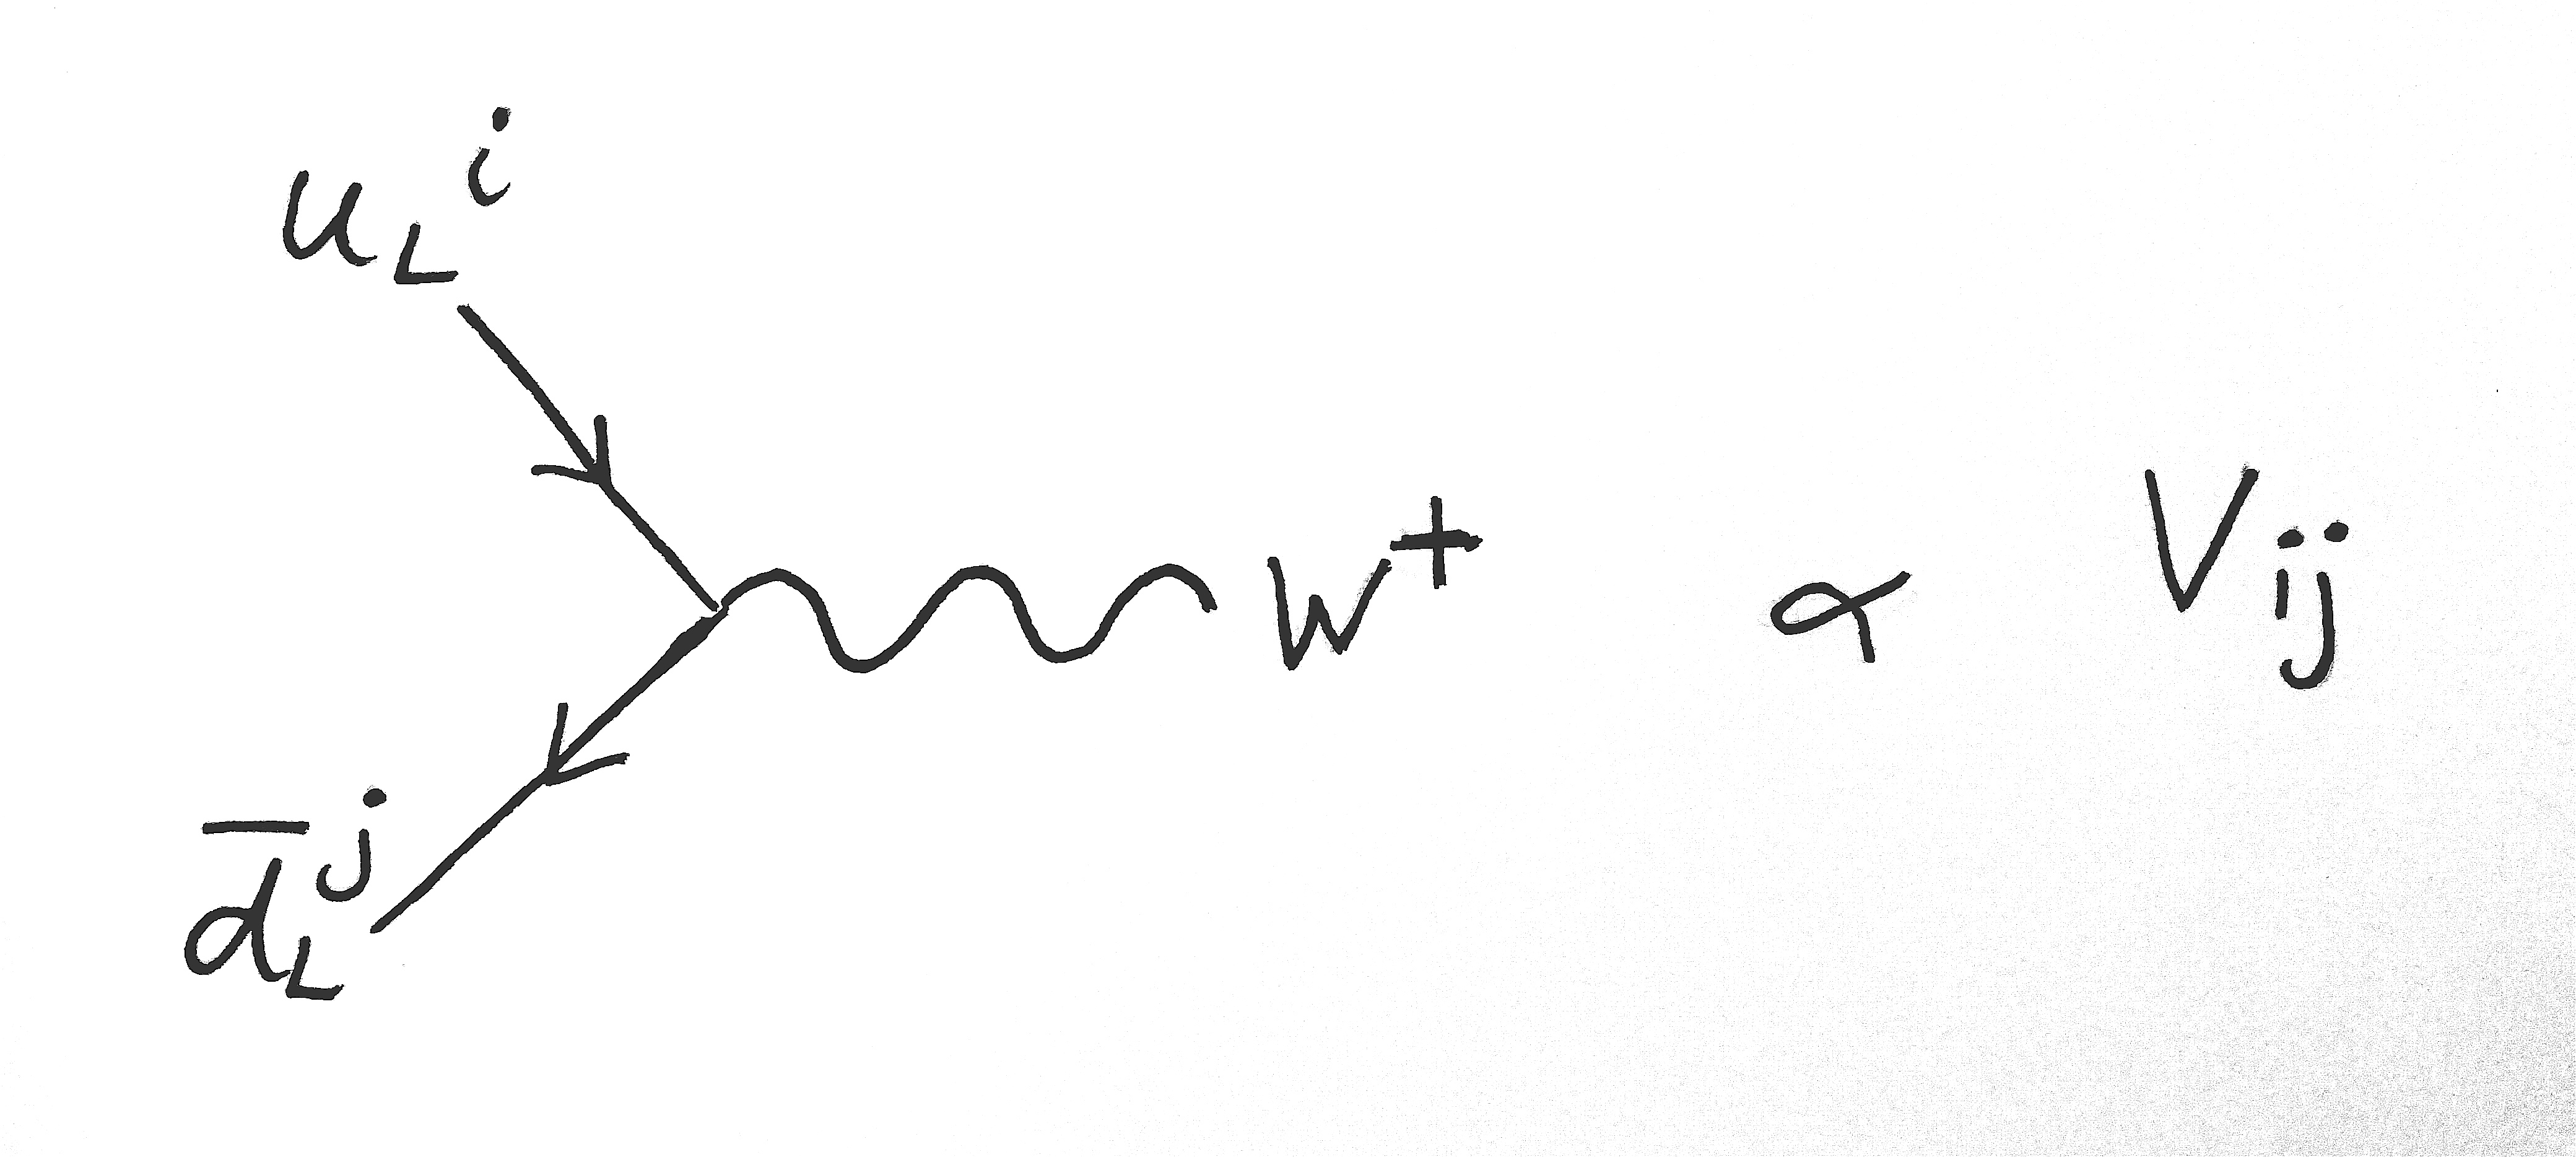
\includegraphics[width=0.5\textwidth]{images/fccc.jpg}
    \vspace{-10pt}
  \end{center}
  \caption{The flavour-changing charged current vertex.}
  \label{fig:fccc}
\end{figure}

The propensity for flavour $i$ to decay into another flavour $j$, is govorned in part by energy constraints and in part by the associated CKM element $V_{ij}$. These interactions at the quark level mediate meson decays, namely leptonic and semileptonic decays, described in section \ref{sec:weakdecays}.

\subsection{The CKM Matrix}

The exact values of the CKM matrix elements are of interest in the search for new physics. The CKM matrix is unitary by construction, however, if we were to discover that the values we measure experimentally do not combine to produce a unitary matrix, this would be evidence that the elements we are measurning infact compose a submatrix of a unitary matrix larger than $3\times 3$. This would imply the presence of further, heavier quark generations.

Another source of interest in the CKM values is CP violation. CP violation is a global symmetry exhibited by $\mathcal{L}_{\text{SM}}-\mathcal{L}_{\text{FCCC}}$, and physically corresponds to a symmetry between particles and antiparticles. CP violation is one of the famous {\it{Sakarov conditions}}, the conditions neccesary for a theory to explain the matter/antimatter asymmetry observed in the universe. CP is generically violated when a parameter of the theory has an imaginary component. As will be shown below, the CKM matrix contains one physical phase, making $\mathcal{L}_{\text{FCCC}}$ a source of CP violation. However, the extent of CP violation in the flavour sector is not sufficient to explain the matter/antimatter asymmetry, so the necessary CP violating processes will likely come from new physics beyond the standard model.


To understand the structure of the CKM, we must first ask how many independent physical parameters there are. If one imagines that $V$ is purely real, then it becomes an $SO(3)$ matrix, which can be parameterised by 3 angles, so there are $N_{\text{real}} = 3$ independent real parameters. A member of $SU(3)$ has 9 independent parameters, so there must be $N_{\text{im}}=N-N_{\text{real}} = 6$ independent phases.

However, we have the freedom to remove some of those phases via a redefinition of the quark fields. $\mathcal{L}_{\text{SM}} - \mathcal{L}_{\text{FCCC}}$ has a global $U(1)^6$ symmetry, a rephasing of each of the 6 quark flavours. One can rephase each flavour without modifying $\mathcal{L}_{\text{SM}} - \mathcal{L}_{\text{FCCC}}$, but with the effect of changing $V$:
\begin{align}
  V \,\,\to \,\,
  \begin{pmatrix}
    e^{-ia} & 0 & 0 \\
    0 & e^{-ib} & 0 \\
    0 & 0 & e^{-ic} \\
  \end{pmatrix}
  V
  \begin{pmatrix}
    e^{id} & 0 & 0 \\
    0 & e^{ie} & 0 \\
    0 & 0 & e^{if} \\
  \end{pmatrix},
\end{align}
where $a,b,c,d,e,f\in \mathbb{R}$. So perhaps one can tune each of these 6 phases to remove all 6 phases in $V$. This is not quite right, we in fact only have the ability to remove 5 of the 6 phases. To see why we can redefine the phases in the following way;
\begin{align}
  V \,\,\to \,\,
  \begin{pmatrix}
    e^{-ia} & 0 & 0 \\
    0 & e^{-i(a+\alpha)} & 0 \\
    0 & 0 & e^{-i(a+\beta)} \\
  \end{pmatrix}
  V
  \begin{pmatrix}
    e^{i(a+\gamma)} & 0 & 0 \\
    0 & e^{i(a+\delta)} & 0 \\
    0 & 0 & e^{i(a+\epsilon)} \\
  \end{pmatrix},
\end{align}
with $\alpha,\beta,\gamma,\delta,\epsilon\in\mathbb{R}$. $a$ is a useless phase - it will always cancel with itself so cannot be used to remove a phase from $V$. Hence, one can remove 5 of the 6 phases by redefining the quark fields, leaving one physical phase in the CKM matrix.

This is can be seen as due to the explicit symmetry breaking property of $\mathcal{L}_{\text{FCCC}}$. Inclusion of $\mathcal{L}_{\text{FCCC}}$ breaks the global $U(1)^6$  symmetry down, $U(1)^6 \to U(1)$, where the broken symmetry is a rephasing of all of the quark flavours by the same amount. This says we can modify $\mathcal{L}_{\text{FCCC}}$ by $N_{\text{broken}} = 5$ independent phases without modifying the rest of the Lagrangian.

So the CKM has 3 real parameters and 1 complex phase. A common parameterisation is
\begin{align}
  V =
  \begin{pmatrix}
    1 & 0 & 0 \\
    0 & \cos\theta_{23} & \sin\theta_{23} \\
    0 & -\sin\theta_{23} & \cos\theta_{23} \\
  \end{pmatrix}
  \begin{pmatrix}
    1 & 0 & \sin\theta_{12}e^{i\delta} \\
    0 & 1 & 0  \\
    -\sin\theta_{13} e^{i\delta} & 0 & \cos\theta_{13} \\
  \end{pmatrix}
  \begin{pmatrix}
    \cos\theta_{12} & \sin\theta_{12} & 0  \\
    -\sin\theta_{12} & \cos\theta_{12} & 0 \\
    0 & 0 & 1 \\
  \end{pmatrix}.
\end{align}
A useful parameterisation for understanding the relative sizes of the CKM elements is due to Wolfenstein. Deifine the Wolfenstein parameter $\lambda = \sin\theta_{12}$, which is know experimentally to be around $\lambda\simeq 0.22$. Then $\cos\theta_{12} = \sqrt{1-\sin^2\theta_{12}} = \sqrt{1-\theta^2} \simeq 1 - \lambda^2/2$. Observing then that $\sin\theta_{23} \sim 0.04 \simeq \lambda^2$ and $\sin\theta_{13} \sim 0.004 \simeq \lambda^3/3$, we can write the matrix as
\begin{align}
  V \simeq
  \begin{pmatrix}
    1 - {1\over 2}\lambda^2 & \lambda & {1\over 3} \lambda^3 e^{i\delta}  \\
    - \lambda & 1 - {1\over 2}\lambda^2 & \lambda^2 \\
    \lambda^3(1-{1\over3} e^{i\delta}) & -\lambda^2 & 1 \\
  \end{pmatrix}
  =
    \begin{pmatrix}
    \order{1} & \order{\lambda} & \order{\lambda^3}  \\
    \order{\lambda} & \order{1} & \order{\lambda^2} \\
    \order{\lambda^3} & \order{\lambda^2} & \order{1} \\
  \end{pmatrix}
\end{align}
There is a clear hierarchy between the values - the CKM matrix is close to the unit matrix. Inter-generational mixing is dominant, dropping from second to first generation is suppressed by $\lambda$, dropping from third to second by $\lambda^2$, and dropping from third to first by $\lambda^3$. The SM supplies no compelling explaination of why this hierarchy exists, it is expected that new physics beyond the SM will supply some natural explaination.

The assumption of unitarity in $V$,
\begin{align}
  V_{ji}^*V_{jk}=\delta_{ik},
  \label{eq:CKMunitarity}
\end{align}
imposes 9 constraints on the CKM elements. Each of these constraints gives a test of the SM, if one of these constraints is found to be violated, this represents evidence of new phyisics. The most studied constraint is given by taking $i=3,k=1$;
\begin{align}
  {V_{ud}V_{ub}^*\over V_{cd} V_{cb}^*} + {V_{td}V_{tb}^* \over V_{cd}V_{cb}^*} + 1 = 0.
\end{align}
This can be visualized as a triangle (known as the {\it{unitarity triangle}}) on the complex plane, as shown in figure \ref{fig:unitaritytriangle_sketch}.

\begin{figure}
  \vspace{-10pt}
  \begin{center}
    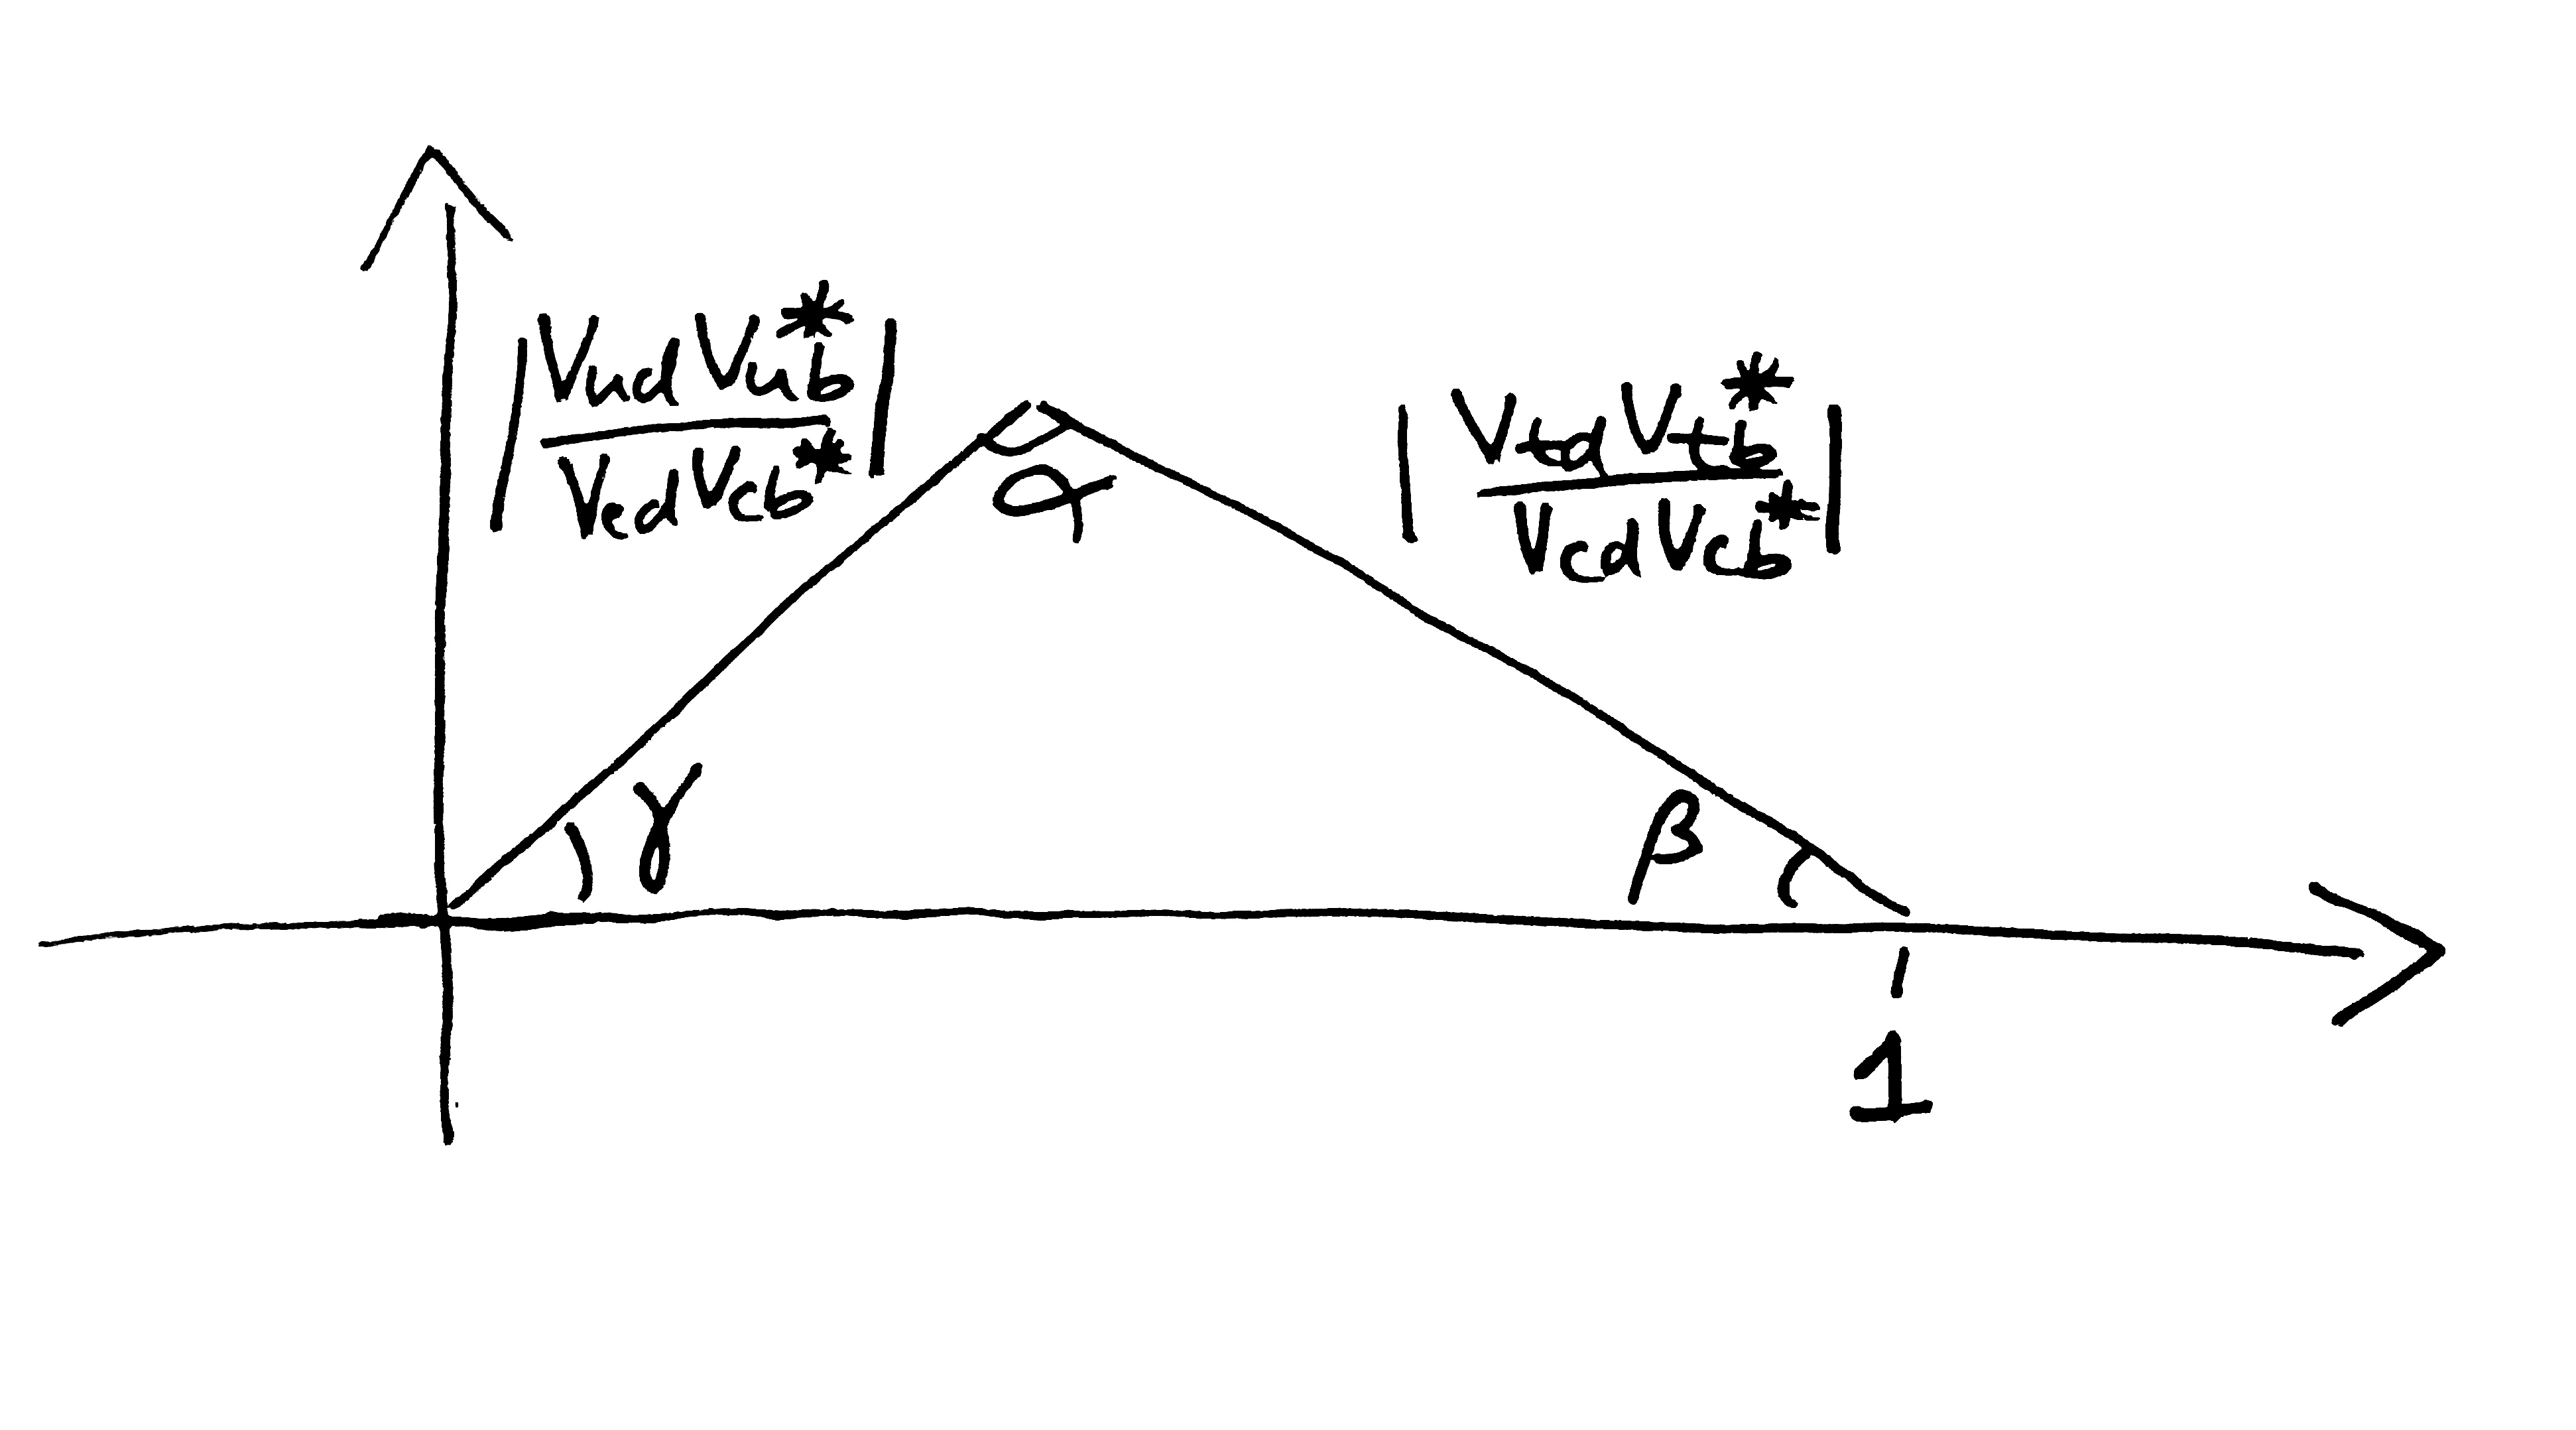
\includegraphics[width=0.7\textwidth]{images/unitaritytriangle_sketch.jpg}
  \end{center}
  \vspace{-25pt}
  \caption{A sketch of the unitarity triangle.}
  \label{fig:unitaritytriangle_sketch}
\end{figure}

For unitarity, the triangle must close, in other words, $\alpha+\beta+\gamma = \pi/2$. Hence, to test the CKM unitarity experimentalists measure these angles
\begin{align}
  \alpha = \arg \left( -{V_{td}V_{tb}^*\over V_{ud}V_{ub}^*}\right) \,,\,
  \beta = \arg \left( -{V_{cd}V_{cb}^*\over V_{td}V_{tb}^*} \right) \,,\,
  \gamma = \arg \left( -{V_{ud}V_{ub}^*\over V_{cd}V_{cb}^*} \right).
\end{align}
The unitarity triangle also contains information about CP-violation from flavour-changing charged currents. The so-called Jarlskog invariant, $J=\sin\theta_{12}\sin\theta_{23}\sin\theta_{31}\cos\theta_{12}\cos\theta_{23}\cos\theta_{31}^2\sin\delta$, a measure of CP-violation, is proportional to the area enclosed by the triangle.

The most recent PDG update \cite{PhysRevD.98.030001} reports the following averages for the measurements of CKM elements;
\begin{align}
  |V| = \begin{pmatrix}
    0.97446\pm 0.00010 & 0.22452\pm 0.00044 & 0.00365\pm 0.00012 \\
    0.22438\pm 0.00044 & 0.97359\substack{+0.00010\\-0.00011} & 0.04214\pm 0.00076 \\
    0.00896\substack{+0.00024\\-0.00023} & 0.04133\pm 0.00074 & 0.999105\pm 0.000032 \\
    \end{pmatrix}.
\end{align}
The averages given here are consistent with unitarity in all avaliable tests. For example, taking \eqref{eq:CKMunitarity} with $i=k=1$, we find $|V_{ud}|^2+|V_{us}|^2+|V_{ub}|^2 = 0.9994\pm 0.0005$. The angles of the unitarity triangle currently satisfy $\alpha+\beta+\gamma = (180\pm 7)\degree$.

\begin{figure}
  \vspace{-10pt}
  \begin{center}
    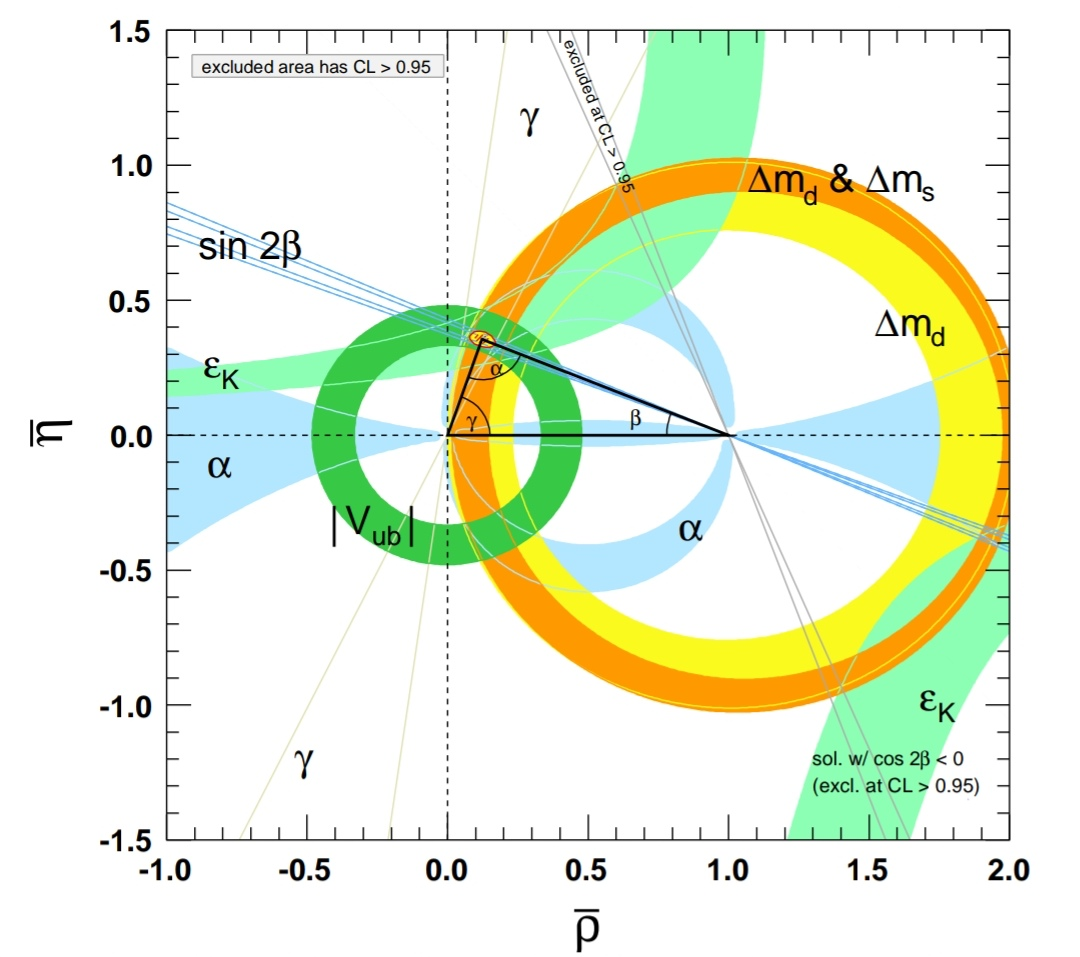
\includegraphics[width=0.7\textwidth]{images/ckmpdg.jpg}
  \end{center}
  \vspace{-25pt}
  \caption{Exclusion regions for the vertices of the CKM triangle from various measurements, coutresy of the most recent PDG update [{\red{!}}]}
  \label{fig:ckmpdg}
\end{figure}

Increasing the precision of CKM determinations are necessary to provide more stringent tests of CKM unitarity.

\subsection{Weak Decays}
\label{sec:weakdecays}

We now move on to the methods of determining CKM elements. At the confinement scale ($\sim$1GeV and below), quarks are confined by QCD in hardons. At these energies, the dynamics of quarks are only experimentally accessable by probing the dynamics of hadrons. CKM matrix elements are determined by studying hadron decays.

First a word on hadrons. Hadrons are broadly categorized into mesons (charged with one valence quark and one valence antiquark) and baryons (three valence quarks). The entirety of this thesis is concerned with mesons. Mesons are categorized in terms of the flavours they are charged under and their representations under the Lorentz group. We use the notation $L^{\pm}$, where $L$ is the meson's spin and $\pm$ denotes it's parity. In this thesis we are concerned mostly with pseudoscalar ($0^-$) and vector ($1^-$) mesons. A deeper discussion on this is postponed until sec. \ref{sec:stronginteractions}.

Weak decays of mesons are categorized according to the final products:
\begin{itemize}
\item
  {\bf{Leptonic}}: $meson \to leptons$.
\item
  {\bf{Semileptonic}}: $meson \to meson + leptons$.
\item
  {\bf{Hadronic}}: $meson \to mesons$.
\item
  {\bf{Oscillation}}: $meson \to meson$.
\end{itemize}

All of these types of decay are dependent on CKM elements so can in principle to be used for studying them. We are most interested in the first two, leptonic and semileptonic, so will give detail of such decays here.

\begin{figure}
  \vspace{-10pt}
  \begin{center}
    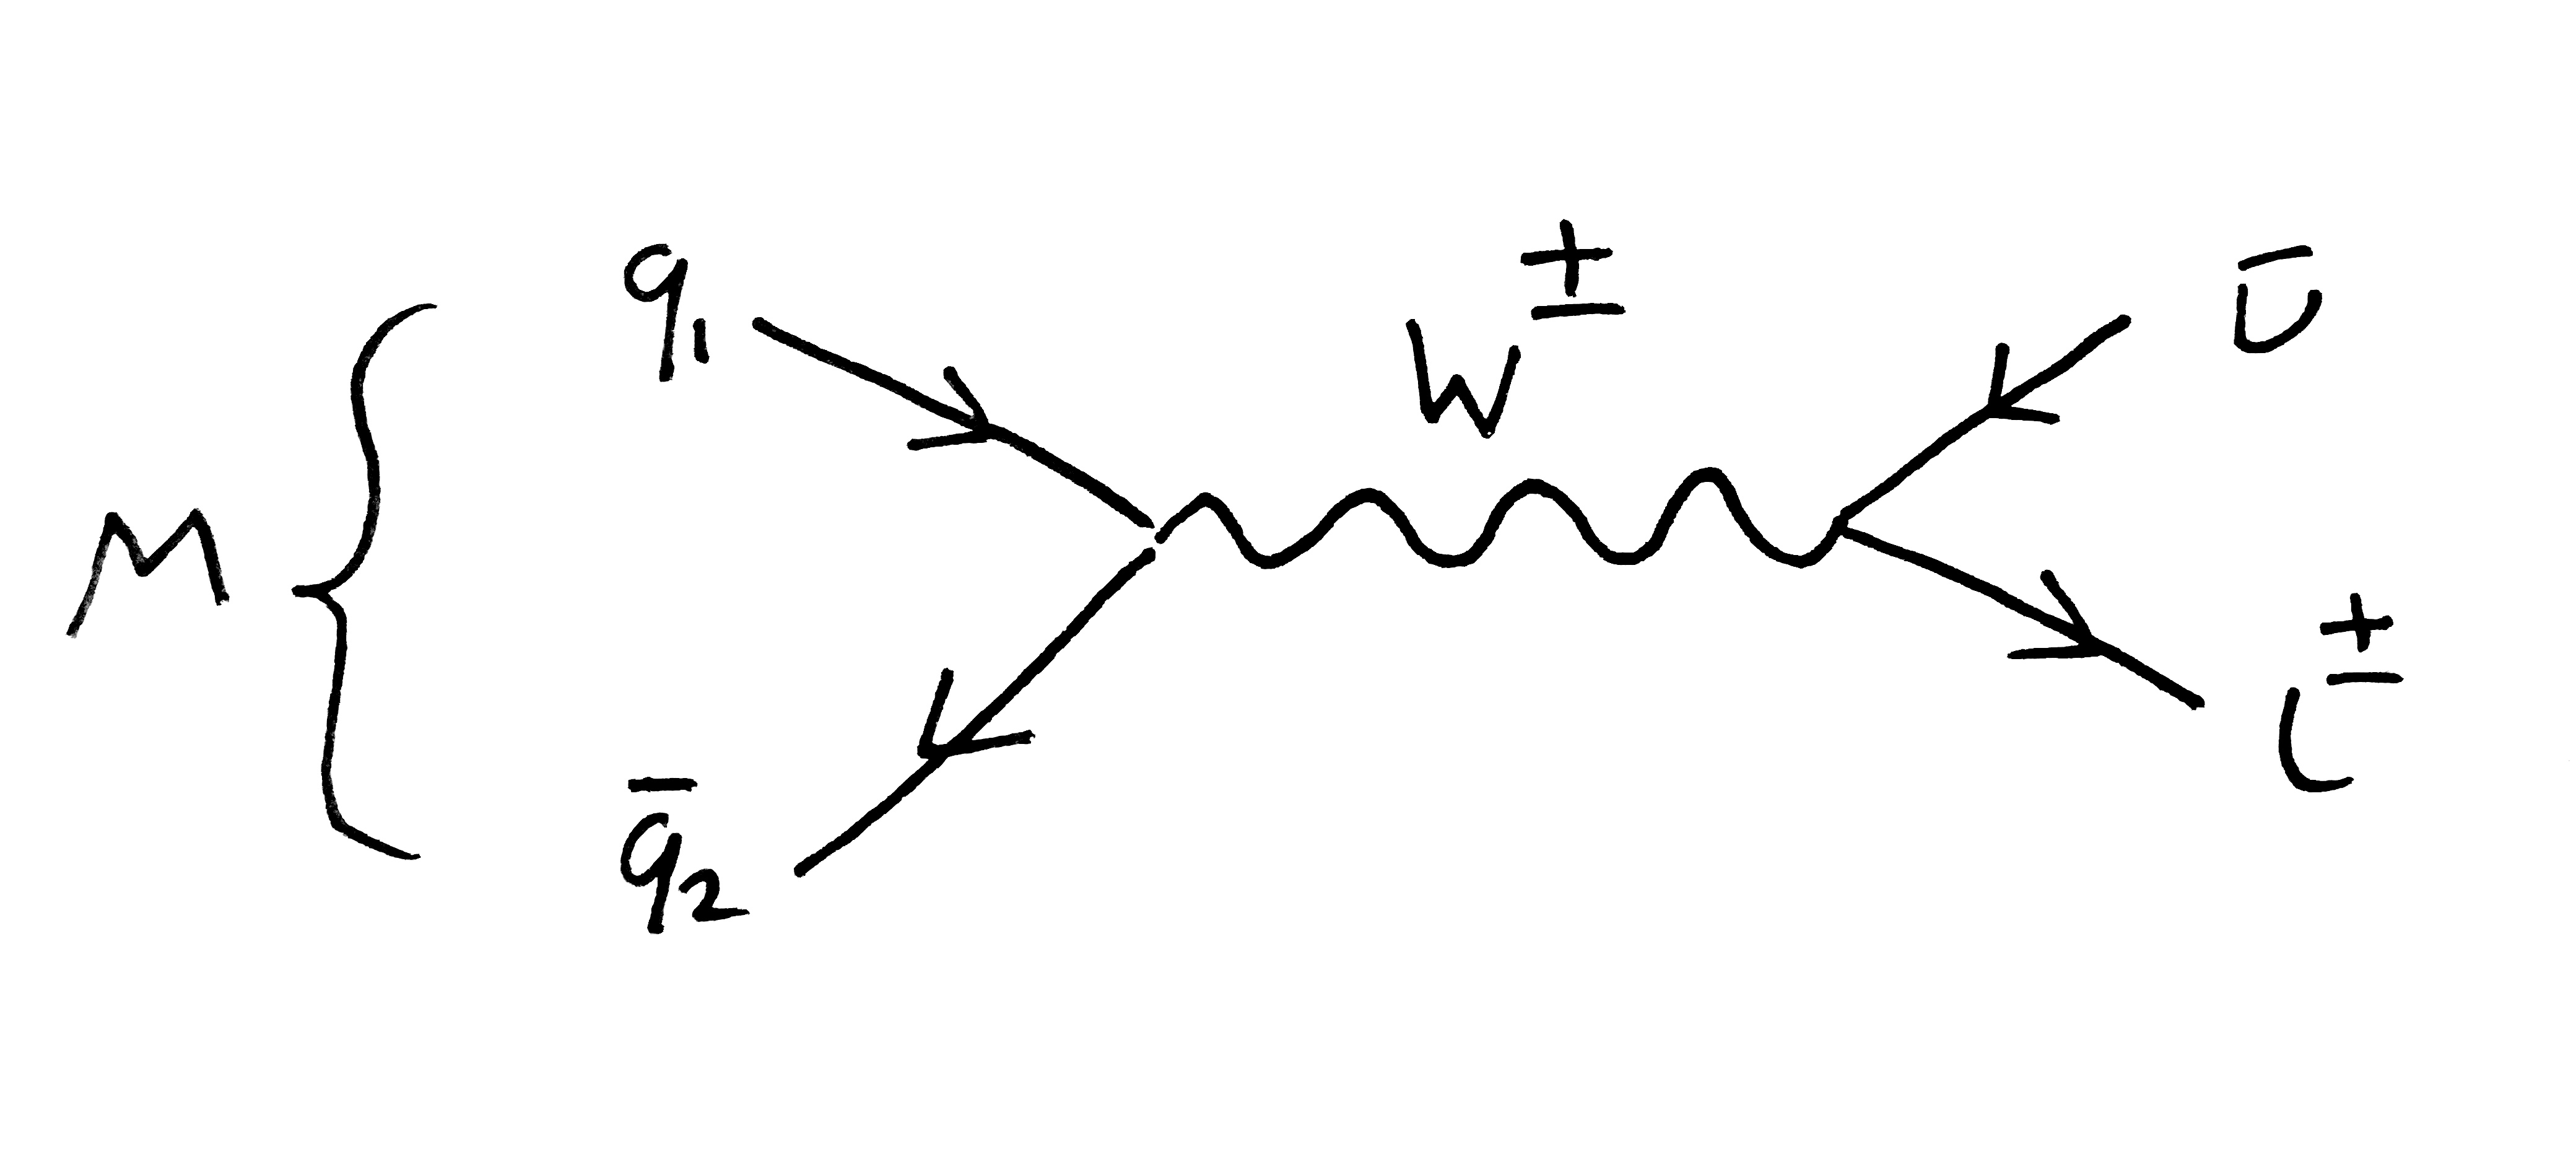
\includegraphics[width=0.6\textwidth]{images/leptonicdecay.jpg}
  \end{center}
  \vspace{-20pt}
  \caption{Leptonic decay of meson $M$ at tree level in the electroweak coupling.}
  \label{fig:leptonicdecay}
\end{figure}

Fig. \ref{fig:leptonicdecay} shows a generic leptonic decay at tree level (in electroweak coupling, virtual quark and gluon lines are implicit). The corresponding amplitude is given by
\begin{align}
\mathcal{M} = \left({ie\over \sqrt{2}\sin\theta_W}\right) V_{q_1q_2} \langle l\bar{\nu} | L^l_{\mu} D_W^{\mu\nu} J_{\nu}^{q_1q_2} | M \rangle,
\end{align}
where $D_{W}$ is the $W^-$ propagator, $|M\rangle$ is the ground state of the meson $M$, and $|l\bar{\nu}\rangle$ is a lepton-antineutrino state. We are using the notation $L^l_{\mu}=L^{kk}_{\mu}$, where $l$ represents the $k$th charged lepton. If the momentum of the meson, $p^2$, is much smaller than the $W$ mass squared, one can integrate out the dynamics of the $W$ to move into the Fermi effective theory \cite{Borasoy:2007yi};
\begin{align}
  \nonumber
 \left({ie\over\sqrt{2}\sin\theta_W}\right)^2 D^{\mu\nu}_W(p^2) &= \left({ie\over\sqrt{2}\sin\theta_W}\right)^2 \left( -ig^{\mu\nu} \over p^2 - M_W^2 \right)
 \\ & = \underbrace{ {i\over M_W^2} \left( ie \over \sqrt{2}\sin\theta_W \right)^2  }_{\equiv -2\sqrt{2}G_F} g^{\mu\nu} + \mathcal{O}\left({p^2\over M_W^4}\right).
\end{align}
Then $\mathcal{M}$ can be factorised;
\begin{align}
  \mathcal{M} \simeq -2\sqrt{2} V_{q_1q_2} \langle l\bar{\nu} | L_{\mu}^l | \Omega \rangle \langle \Omega | J^{q_1q_2\, \mu} | M \rangle.
\end{align}
$\langle \Omega | J^{q_1q_2}_{\mu}| M \rangle$ is a non-perturbative quantity, since it concerns the transitions of a strongly coupled bound state (QCD at the confinement scale). We know that it has a lorentz index $\mu$, and the only Lorentz vector in the system is the meson's 4-momentum $p_{\mu}$. So we define
\begin{align}
  \langle\Omega | J_{q_1q_2}^{\mu} | M \rangle = p^{\mu} f_M,
\end{align}
where $f_M$ is a Lorentz invariant known as the {\it{decay constant}} of the meson $M$, and encodes all non-perturbative information in the amplitude.

By taking the modulus squared of $\mathcal{M}$, and integrating over all allowed momenta of the final state, one finds the decay rate of the process:
\begin{align}
  \Gamma(M\to l\bar{\nu}) = {G_F^2\over 8\pi} f_M^2 m_l^2 M_M \left( 1 - {m_l\over M_M^2} \right)^2 |V_{q_1q_2}|^2,
\end{align}
In order to find $|V_{q_1q_2}|$, one requires both a measurement of $\Gamma(M\to l\bar{\nu})$, and a value for $f_M$. $f_M$ can be computed in a Lattice QCD calculation.

%\begin{wrapfigure}{R}{0.55\textwidth}
\begin{figure}
  \vspace{-10pt}
  \begin{center}
    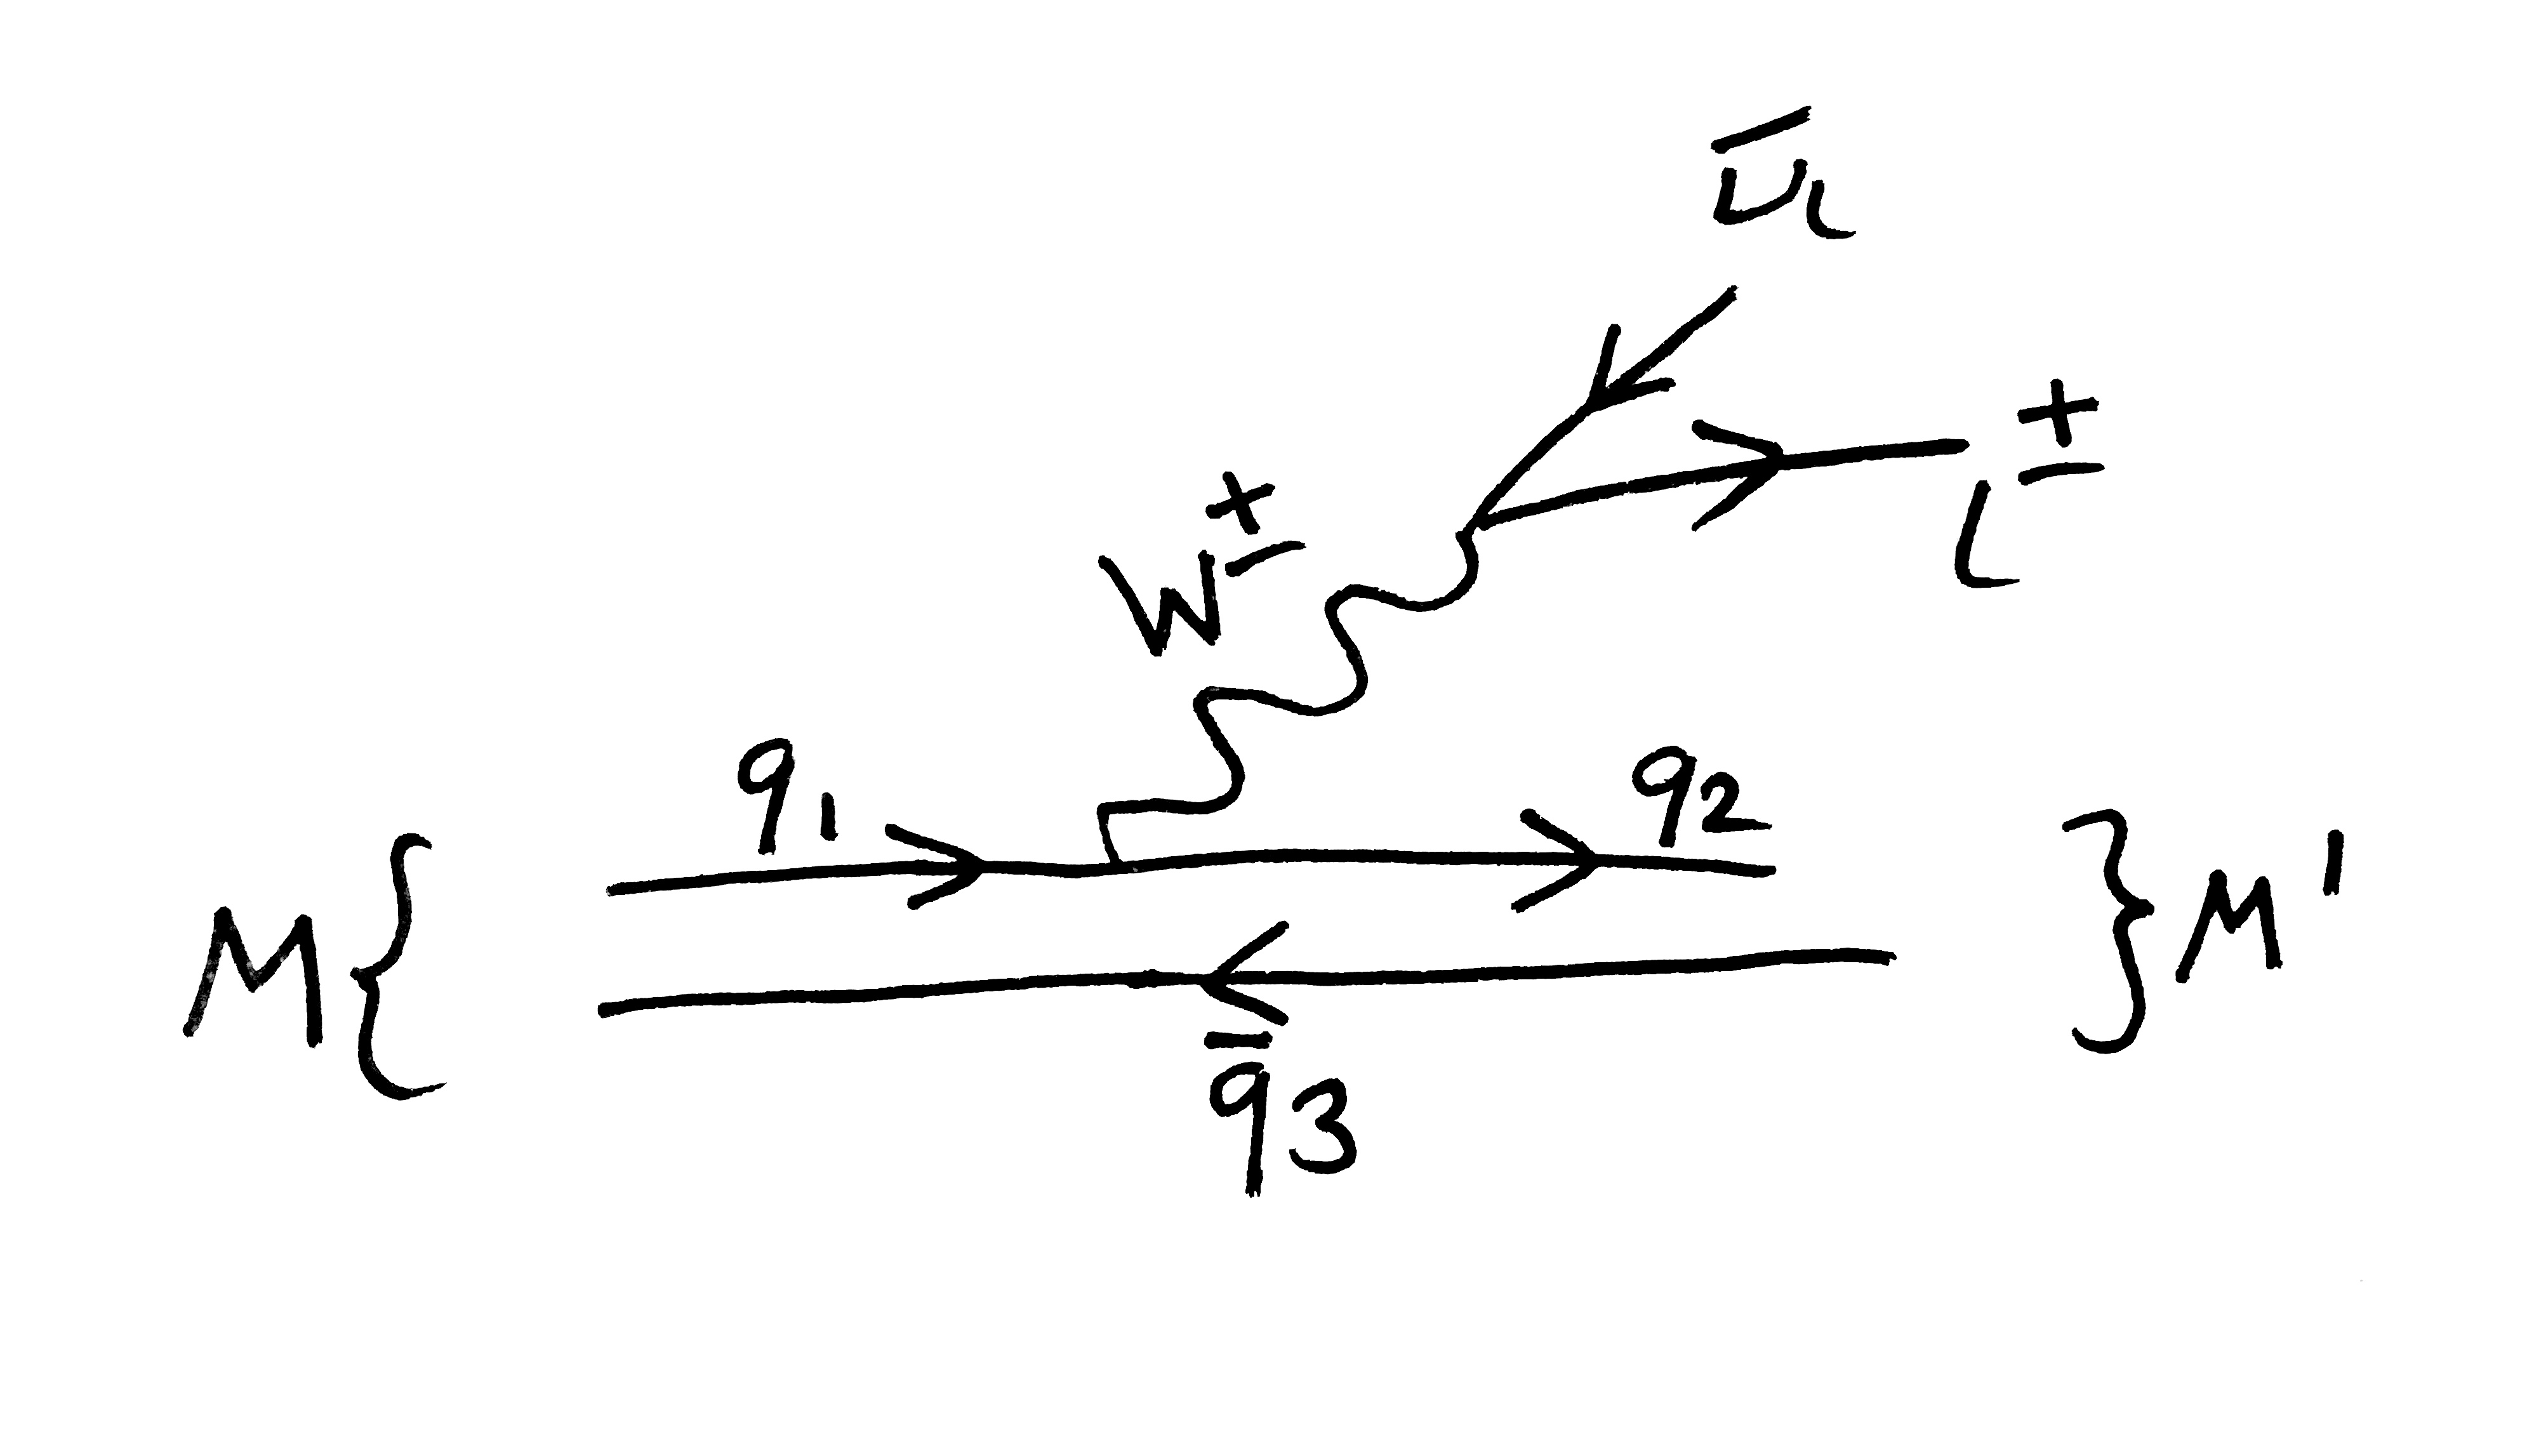
\includegraphics[width=0.6\textwidth]{images/semileptonicdecay.jpg}
  \end{center}
  \vspace{-30pt}
  \caption{Semileptonic decay, $M\to M'l\bar{\nu}$, at tree level in electroweak coupling.}
  \label{fig:semileptonicdecay}
\end{figure}
%\end{wrapfigure}

A similar story accompanies semileptonic decays. At tree level in the electroweak coupling, a typical semileptonic decay is depicted in fig. \ref{fig:semileptonic}. The amplitude is given by
\begin{align}
  \nonumber
  \mathcal{M} & = \left( { ie \over \sqrt{2} \sin\theta_W }\right) V_{q_1q_2} \langle M', l\bar{\nu} | J_{\mu}^{q_1q_2} D_W^{\mu\nu} L^l_{\nu} | M \rangle \\
  \nonumber
  & \simeq -2\sqrt{2} G_F V_{q_1q_2} \langle M', l\bar{\nu} | J_{\mu}^{q_1q_2} L^{l\, \mu} | M \rangle \\
  & \simeq -2\sqrt{2} G_F V_{q_1q_2} \langle l\bar{\nu} | L^{l\,\mu} | \Omega \rangle \langle M' | J_{\mu}^{q_1q_2} | M \rangle
  \label{eq:semileptonic}
\end{align}
where on the second line we have integrated out the $W$ propagator in using the same expansion as in the leptonic case, and on the third line we have factorised the QCD part from the electroweak part. The matrix element $\langle M' | J_{\mu}^{q_1q_2} | M \rangle$ is a non-perturbative quantity. Unlike in the previous case, there are a number of ways one can choose to parameterise this matrix element, and appropriate choices vary depending on the quantum numbers of $M$ and $M'$. Of interest to us are the cases where $M$ is a pseudoscalar meson $0^-$, and $M'$ is either pseudoscalar or vector $1^-$.

In the {\bf{pseudoscalar$\to$pseudoscalar}} case, only the vector component of the current survives in the matrix element, $\langle M' | J_{\mu}^{q_1q_2} | M \rangle = \langle M' | V_{\mu}^{q_1q_2} | M \rangle$, $\langle M' | A_{\mu}^{q_1q_2} | M \rangle$ vanishes since this does not respect the parity invariance of QCD. The most popular parameterisation of $\langle M' | J_{\mu}^{q_1q_2} | M \rangle$ is
\begin{align}
  \langle M' | V_{\mu}^{q_1q_2} | M \rangle = f_+(q^2) \left[ P_{\mu} + p_{\mu} - {M^2-m^2\over q^2} q_{\mu} \right]  + f_0(q^2) {M^2-m^2\over q^2} q_{\mu} 
\end{align}
$f_0(q^2)$ and $f_+(q^2)$, known as the scalar and vector form factors, encode all non-perturbative information. We now have non-perturbative functions of $q^2$ rather than a single number. $q^2$, the momentum carried away from the meson by the $W$, has an The allowed range of values if the final states are on-shell;
\begin{align}
  m_l^2 \leq q^2 \leq (M-m)^2.
\end{align}
By integrating $|\mathcal{M}|^2$ over all final lepton and neutrino momenta, one finds a differential decay rate.
\begin{align}
  {d\Gamma\over dq^2}(M\to M'l\bar{\nu}) =& \eta_{\text{EW}} { G_F^2 |V_{q_1q_2}|^2\over 24 \pi^3 M^2 } \left( 1 - {m_l^2\over q^2}\right)^2 |{\bf{p}}| \,\,\times \\
  \label{eq:branchingfraction}
  &\left[ \left( 1 + {m_l^2\over 2q^2}\right) M^2 |{\bf{p}}|^2 f_+^2(q^2) + {3m_l^2\over 8q^2} (M^2-m^2)^2 f_0^2(q^2) \right]. \nonumber
\end{align}
$\eta_{\text{EW}}$ is the electroweak correction, due to diagrams involving an exchange of a photon or a $Z$-boson alongside the $W$ betweent the meson and leptons. ${\bf{p}}$ is the final meson state ($M'$) spacial momentum. Once again, to deduce $|V_{q_1q_2}|$, one requires both the decay rates $d\Gamma/dq^2$, and the form factors $f_0(q^2)$,$f_+(q^2)$. To precisely determine the form factors requires a Lattice QCD calculation.

In the {\bf{pseudoscalar$\to$vector}} case, both the vector and axial-vector components of the current survive in the matrix element. A common choice of parameterisation is
%% \begin{align}
%%   \langle M' | V^{\mu} | M \rangle &= {2iV(q^2)\over M+m} \epsilon^{\mu\nu\rho\sigma} \epsilon_{\nu}^* p_{\rho}P_{\sigma} \\
%%   \langle M' | A^{\mu} | M \rangle &= 2mA_0(q^2) {\epsilon^*\cdot q\over q^2} q^{\mu} + (M+m)A_1(q^2)\left[ \epsilon^{*\,\mu} - {\epsilon^*\cdot q\over q^2} q^{\mu} \right] \\
%%   \nonumber
%%   &- A_2(q^2) {\epsilon^*\cdot q\over M + m} \left[ P^{\mu} + p^{\mu} - {M^2-m^2\over q^2} q^{\mu} \right].
%% \end{align}
A common choice of parameterization is
\begin{align}
  \langle M'(\epsilon)| V_{q_1q_2}^{\mu} | M \rangle &= i \sqrt{Mm}\, h^s_V(w) \epsilon_{\mu\nu\alpha\beta} \,\epsilon^{*\nu} v'^{\alpha} v^{\beta}, \\
  \langle M'(\epsilon)| A_{q_1q_2}^{\mu} | M \rangle &= \sqrt{Mm} \, [ h^s_{A_1}(w) (w+1) \epsilon^*_{\mu} - \\ \nonumber
    h^s_{A_2}(w)& \,\epsilon^*\cdot v \,v_{\mu} - h^s_{A_3}(w) \,\epsilon^*\cdot v \, v'^{\mu} ].
\end{align}
$v = P/M$ and $v' = p/m$ are the 4-velocities of $M$ and $M'$ respectively. $\epsilon$ is the polarization of the vector meson $M'$. $w = v\cdot v'$ is known as the recoil parameter, this is an alternative to $q^2$ often used in heavy quark effective theory. $h_V(w),h_{A_0}(q^2),h_{A_1}(q^2)$, and $h_{A_2}(q^2)$ are the form factors accounting for the non-perturbative physics. The decay rate is given by
\begin{align}
  {d\Gamma \over dw}(M\to M' l\bar{\nu}) = {G_F^2 m^3 | \eta_{\text{EW}} V_{q_1q_2} |^2 \over 4\pi^3 } (M-m)^2 \sqrt{w^2-1} \, \chi(w) |\mathcal{F}(w)|^2,
\end{align}
where $\mathcal{F}(w)$ is a linear combination of the form factors, and $\chi(w)$ is a known function of $w$.

At the zero recoil point, where $q^2$ is maximized at $q^2_{\text{max}} = (M-m)^2$, (correpsonding to $w=1$), a single form factor contributes
\begin{align}
  \mathcal{F}(1) = h_{A_1}(1).
\end{align}
However the differential decay rate vanishes at $w=1$. A common approach to determine $|V_{q_1q_2}|$, for example used to find $|V_{cb}|$ via the $B\to D^*l\bar{\nu}$ decay, is to find $|\mathcal{F}(1)V_{cb}|^2$ at zero recoil by extrapolating from experimental data at non-zero recoil, and combining this with a lattice QCD determination of $h_{A_1}(1)$.

\subsection{$|V_{cb}|$}

The family of weak decays that have attracted the most attention are decays of $B$ mesons (pseudoscalar mesons containing a valence $b$ and $u,d,s$ or $c$ quark). The $B$ meson decays into a rich veriety of decay products. It is the heaviest quark flavour that can be found in hadrons. The only heavier quark, the top quark, has a mass far above the confinement scale, so does not feature as a valence quark in hadrons.

The $b$ can decay into either a charm or an up quark via the flavour changing charged current. In this thesis we are interested in the $b\to c$ transition, with an amplitude proportional to the CKM element $|V_{cb}|$. In this section we give a breif overview of how this is calculated and the value's current status.

$B$ meson decays can be measured in a number of experiments. There are two so-called $b$-factories, the Belle (II) experiment at the KEKB collider in Japan, and the BaBar experiment at the PEP-II collider at SLAC laboratory in the US. These are $e^+e^-$ colliders, that collide with an energy tuned to the mass of the $\Upsilon(4s)$, an excited state of the $\Upsilon$ meson (a $1^-$ state with $\bar{b}b$ valence quarks). The $\Upsilon(4s)$ has a large branching fraction into a $B\bar{B}$ pair, the decays of these can be measured with large statistics. $B$ decays can also be measured in proton colliders, like the LHCb experiment at CERN. Measurements from LHCb have poorer statistics but cover a larger range of the phase space of final states, due to the variance of momenta in the initial state protons.

So far 3 approaches to determining $|V_{cb}|$ have been carried out.
\begin{itemize}
\item
  $B\to D^* l\bar{\nu}$ decay rate measurements are extrapolated to zero recoil to determine $|V_{cb}h_{A_1}(1)|$. Then dividing out $h_{A_1}(1)$ from a Lattice calculation, one finds $|V_{cb}|$.
\item
  $B\to D l\bar{\nu}$ decay rates are measured throughout $q^2$, and combined with $f_0(q^2)$ and $f_+(q^2)$ from lattice calculations.
\item
  $B\to X_c l\bar{\nu}$ decay rates are measured (where $X_c$ is all possible charmed final state mesons), this is used to constrain elements in the operator product expansion, a method first devised in \cite{Bigi:1996si,Hoang:1998hm}.
\end{itemize}
The first two are referred to as {\it{exclusive}} and the third {\it{inclusive}}. A selection of the most accurate examples of each method of determination is given in figure \ref{fig:Vcb_plot}.
\begin{figure}
  \vspace{-10pt}
  \begin{center}
    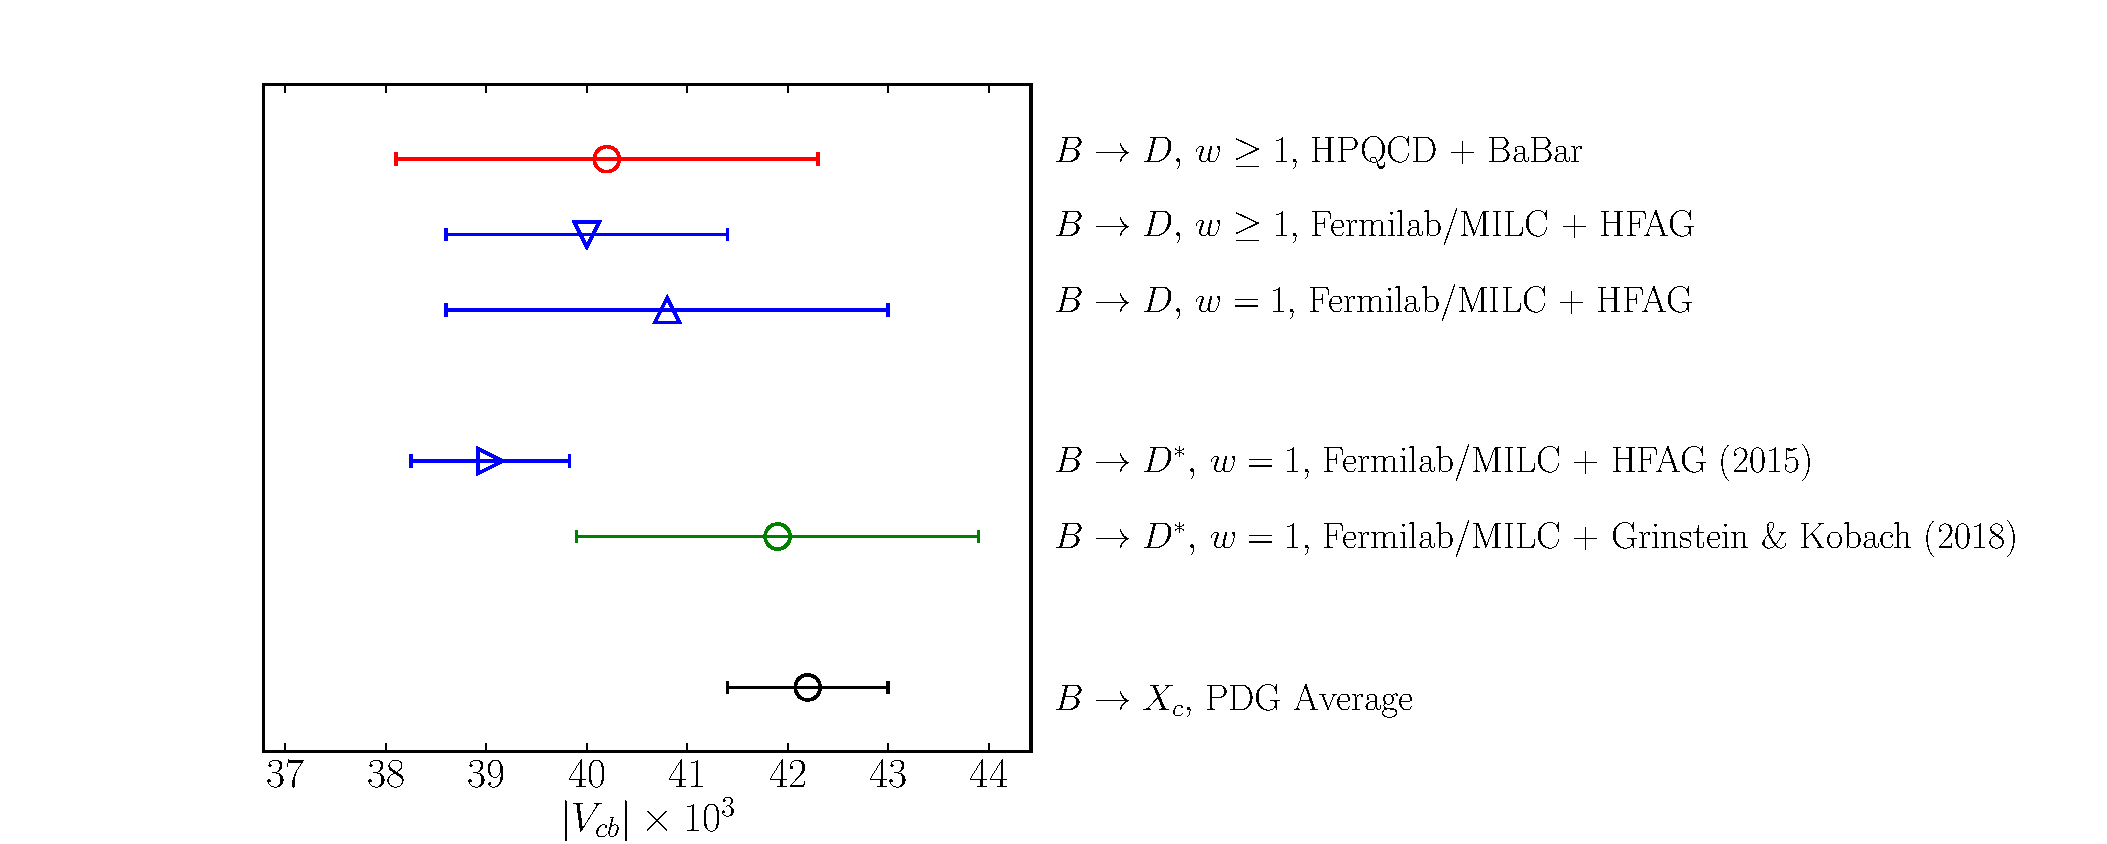
\includegraphics[width=1.0\textwidth]{images/Vcb_plot.pdf}
  \end{center}
  \vspace{-20pt}
  \caption{Different determinations of $|V_{cb}|$. Points labelled $w=1$ are determinations from extrapolating measurements of decay rates to the zero recoil point, and combined with a lattice determination of the form factor at zero recoil. Points labelled $w\geq 1$ are results from using a combination of both branching fractions and lattice form factors through some range of $w$. The first name mentioned in the labels give the source of the lattice form factors, and the second gives the source of the experimental data (e.g. the HPQCD$+$BaBar point used form factors from the HPQCD collaboration and data from the BaBar experiment. The highest point is from \cite{Na:2015kha}, the second and third highest from \cite{Lattice:2015rga}, fourth from \cite{Bailey:2014tva}, fifth from \cite{Grinstein:2017nlq}. The bottom point is from the PDG \cite{PhysRevD.98.030001}, using data from the ALPEPH \cite{BUSKULIC1995236}, Belle \cite{Abe:2001yf}, BaBar \cite{Aubert:2008yv,Aubert:2009ac}, and CLEO \cite{Bartelt:1998dq} experiments.
\label{fig:Vcb_plot}}
\end{figure}

This tells a story of the recent history of $|V_{cb}|$. Determinations from $B\to Dl\nu$ have been consistent but not as precise as via the other two methods. Until recently, there was a $3\sigma$ tension between determinations from the $B\to D^* l\nu$ decay, and inclusive decays. This was on it's way to being resolved when concern was raised about the method of extrapolating experimental data for $B\to D^*l\bar{\nu}$ decay rates to the zero recoil point ($w=1$).

The Heavy Flavour Averaging Group HFAG (Now HFLAV) determination of $|\eta_{\text{EW}}V_{cb}h_{A_1}(1)|$ in 2015 parameterised the form factors in the extrapolation using the CLN parameterisation (defined in section \ref{sec:formfactor_params}). It has become clear that the constraints the CLN parameterisation imposes on the form factors are not justified. In \cite{Bigi:2017njr,Grinstein:2017nlq}, the results of an extrapolation using the CLN parameterisation were compared to results from a more general, model independent parameterisation, the BGL parameterisation. It was found that they differed by $3.5\sigma$. Since the BGL makes less assumptions, one may consider this the more reliable result.

The $|V_{cb}|$ result using BGL to extrapolate the decay rates is given in the green point on fig. \ref{fig:Vcb_plot}. Hence, if this work is to be trusted, the long-standing $|V_{cb}|$ tension has been resolved.

There are however a number of other reasons to be interested in studying $|V_{cb}|$, namely improving it's precision. It is currently the least precisely determined element of the CKM matrix. It constrains one side of the unitarity triangle via the ratio $|V_{ub}|/|V_{cb}|$, so it is the bottleneck for precise tests of CKM unitarity. It is also a dominant uncertainty in the determination of the $CP$-violation parameter $\epsilon_K$ (that is currently at tension between the SM and experiment, see for example \cite{Bailey:2018feb} where a $4\sigma$ tension is reported).

A dominant motivation for the work presented in this thesis is the quest for a more precise determination of $|V_{cb}|$. The main results are form factors for $B_s\to D_s l\bar{\nu}$ and $B_s\to D_s^* l\bar{\nu}$. The benefit of these determinations are two-fold. Firstly, they can be combined with future experimental measurements of $B_s\to D_s^{(*)}l\bar{\nu}$ decays for a new $|V_{cb}|$ determination. Increasing the number of independent determinations of $|V_{cb}|$ makes each result more robust. Secondly, they demonstrate that our approach in the lattice calculations work well and can therefore be applied to $B\to Dl\bar{\nu}$ and $B\to Dl\bar{\nu}$ form factors in the future.

\subsection{Flavour Anomalies}

The SM can be tested from studying semileptonic decays more directly, without any consideration of CKM elements. CKM-independent observables can be constructed by taking ratios of branching fractions for decays with common CKM dependence. Then, form factors from lattice QCD can be used to form pure SM predictions of these ratios, and compared to purely experimental measurements of those ratios. Such comparisons have uncovered a number of tensions between the SM and experiment.

The ratios are defined by
\begin{align}
	R(X) = {\mathcal{B}(B_q\to X_q \tau \nu_{\tau}) \over {1\over 2}\left[\mathcal{B}(B_q\to X_q e \nu_e) + \mathcal{B}(B_q\to X_q \mu \nu_{\mu}) \right]}
\end{align}
where $X_q$ is any meson with valence quark content $x\bar{q}$. Branching fractions $\mathcal{B}(\alpha\to \beta)$ are equal to $\Gamma(\alpha\to \beta)/\Gamma(\alpha\to \{\gamma_i\})$ where $\gamma_i$ are all possible final states. The numerator and denomenator will have the same power of $|V_{bx}|$, so cancel in the ratio.

$R(D^*)$ contains a $~2.1\sigma$ discrepancy \cite{Aaij:2015yra}:
\begin{align}
	R(D^*)|_{\text{SM}} = 0.252(3) \text{ , } R(D^*)|_{\text{LHCb}} = 0.336(27)_{sys}(30)_{stat}
\end{align}
The issue is similarly present for $R(D)$ \cite{Monahan:2017uby}:
\begin{align}
	R(D)|_{\text{SM}} = 0.299(7) \text{ , } R(D)|_{\text{exp}} = 0.391(28)_{sys}(41)_{stat}
\end{align}
where in this case $R(D)|_{\text{expt}}$ is a world average of experimental values. Our eventual study of $B\to Dl\nu$ will produce a new standard model determination of $R(D)$, helping shed light on the issue.
\\ \\
\begin{figure}
  \begin{center}
    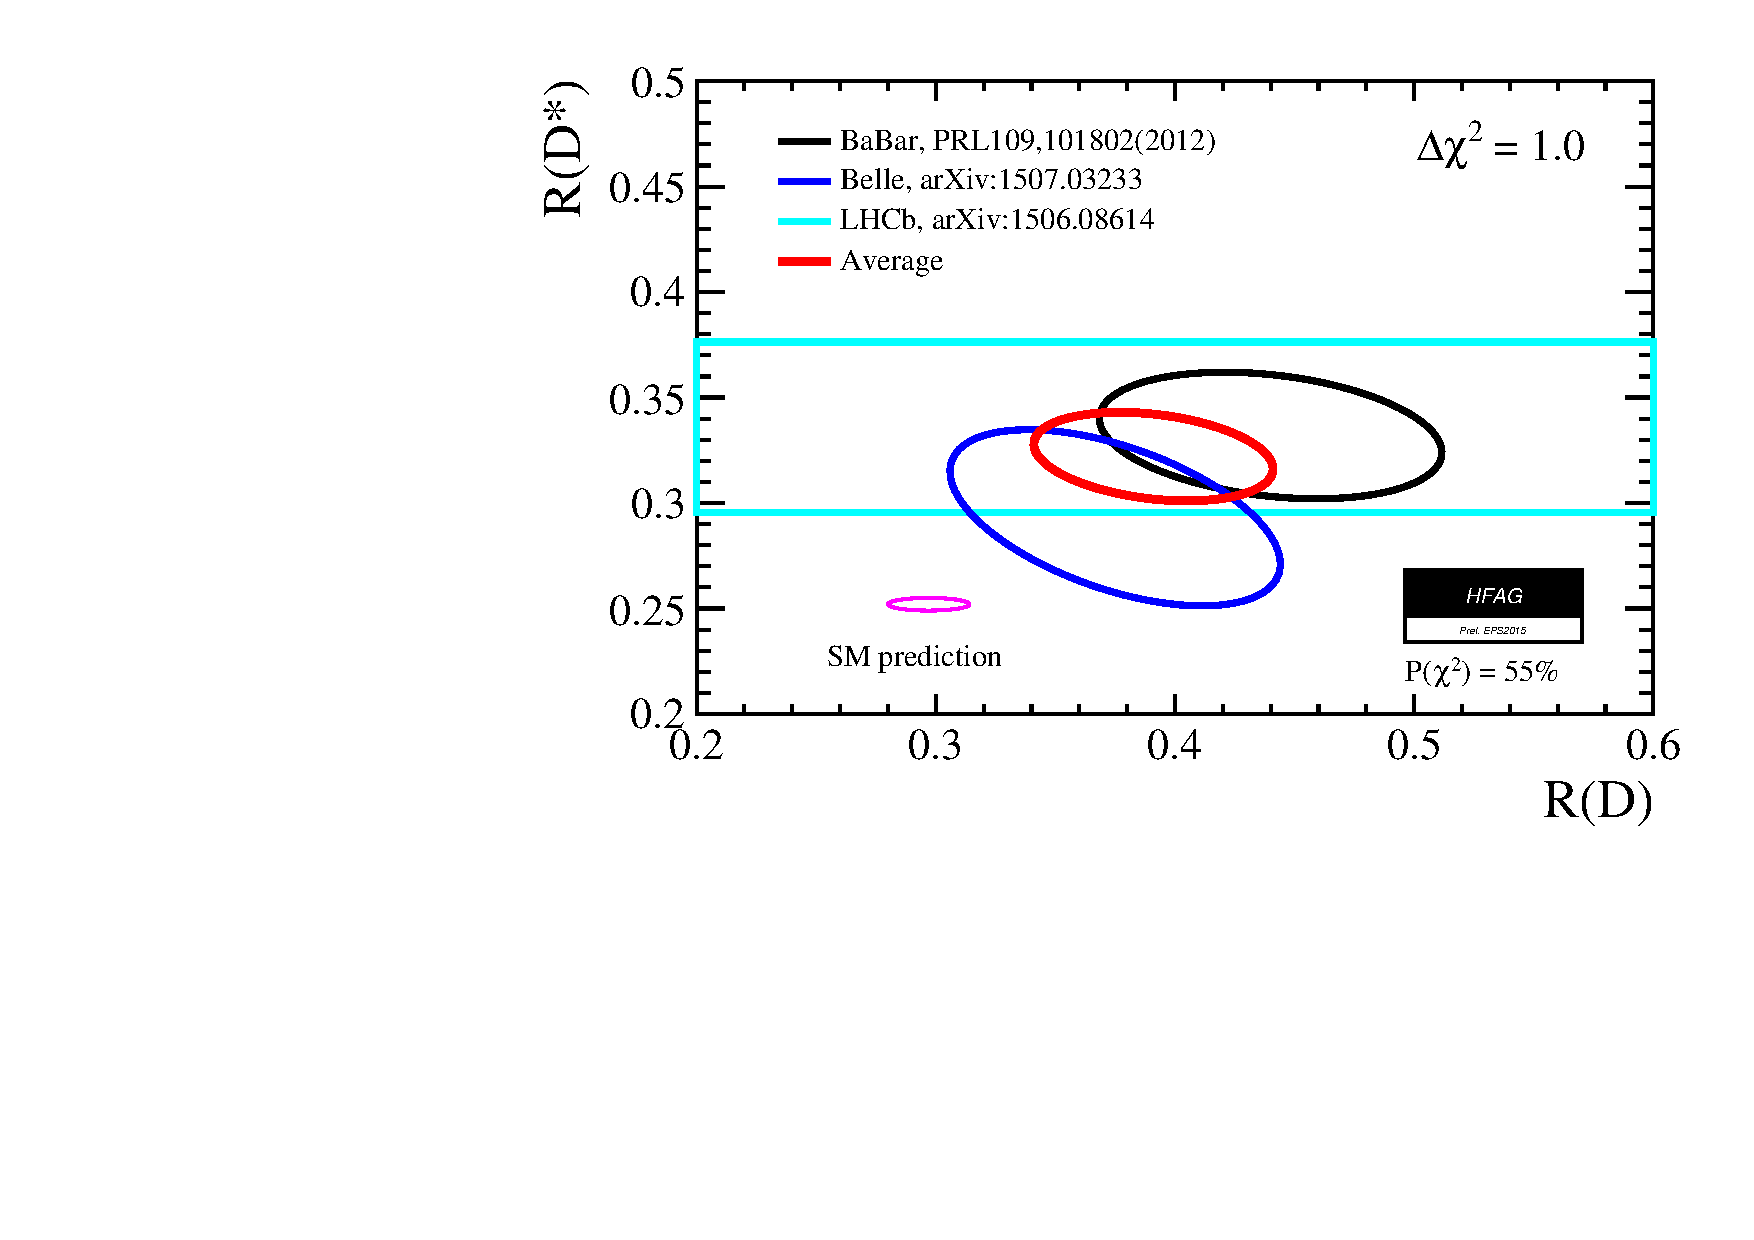
\includegraphics[width=
   0.8\textwidth]{images/rdrds_eps15.pdf}
  \end{center}
  \caption{$R(D)/R(D^*)$ determinations from standard model and experiment \cite{HFAG}}
  \label{fig:semileptonic}
\end{figure}
%A natural question to ask is: is there an analagous tension in related channels, like $B_s\to D_s l\nu$? There is not yet any experimental data for this decay, but the current best standard model determination is given by ${\mathcal{B}(B_s\to D_s \tau \nu_{\tau}) / \mathcal{B}(B_s\to D_s l \nu_l)} |_{\text{SM}} = 0.314(6)$.
\\ \\
Besides these, there are also tensions in the quantitites \cite{Altmannshofer:2017yso}:
\begin{align}
	R'(K^{(*)}) = {\mathcal{B}( B\to K^{(*)}\mu^+\mu^-)\over \mathcal{B}( B\to K^{(*)} e^+e^-)}
\end{align}
All of the above anomalies are suggestive of lepton flavour violating effects. Various BSM models have been suggested; hot topics include Leptoquarks, $Z'$ models, and partial compositeness \cite{Altmannshofer:2017yso}.

